\section{Protocolli di routing}
Quando un pacchetto arriva ad un router ci serve capire quale strada fargli prendere in modo da ottimizzare un qualche parametro di costo.
Questo problema si viene a creare perché i router spesso sono connessi a più di un altro router, quindi i percorsi che il pacchetto può prendere sono molteplici.
Ogni router ha in se memorizzata una tabella di routing che associa ad ogni range di indirizzi l' interfaccia verso la quale instradare i pacchetti provenienti da quella sottorete.

I protocolli di routing si dividono in due macro-famiglie:
\begin{itemize}
    \item link space
    \item distance vector
\end{itemize}
entrambi perseguono però la ricerca del path \emph{ottimo}.

Baseremo tutti i nostri ragionamenti sulla astrazione della rete come grafo, cioè un insieme di nodi collegati da archi.

Quando si parla di ottimale quindi si cerca di ottimizzare rispetto ad un criterio che chiameremo costo.
Possiamo modellare che ogni arco abbia un proprio costo di attraversamento, oppure possiamo pensare che ogni arco abbia costo unitario; nel primo caso si va a minimizzare la somma dei costi degli archi attraversati, nel secondo caso si minimizza il numero di hop!
Inoltre questi costi possono anche essere variabili nel tempo, per esempio supponiamo che il costo sia proporzionale al livello di congestione dell' arco.

Si potrebbe richiedere anche l' ottimizzazione di più di un parametro, in tal caso si sfruttano techiche di ottimizzazione multi-obiettivo come:
\begin{itemize}
    \item linearizzazione del problema
    \item somma pesata degli obiettivi
\end{itemize}

Si cerca sempre un compromesso in quanto la ricerca del path deve essere eseguita velocemente per non aggiungere latenza.

\subsection{Tassonomia dei protocolli di routing}
Possiamo avere una distribuzione tra:
\begin{itemize}
    \item algoritmi globali: i router conoscono la completa topologia della rete, dei costi degli archi.
    Fanno parte della famiglia link state
    
    \item algoritmi distribuiti: i router conoscono solo i vicini ai quali sono collegati ed i pesi di questi collegamenti.
    Serve quindi una computazione iterativa con scambio di informazioni tra vicini.
    Fanno parte della famiglia distance vector
\end{itemize}
oppure in:
\begin{itemize}
    \item static: si usano quando le route cambiano poco spesso e non è quindi necessario modificare i percorsi molto spesso
    
    \item dynamic: le route cambiano velocemente, si ha quindi un update periodico in risposta al cambio dei costi
\end{itemize}

\subsection{Link state}
\subsubsection{Algoritmo di Dijkstra}
Data la topologia intera della rete ed i costi degli archi possiamo usare l' algoritmo di Dijkstra per costruire le shortest path per ogni destinazione.
La complessità è $O(n^2)$ ma ci sono anche implementazioni $O(n\log{n})$.

Soffre di un piccolo inconveniente: se i costi sugli archi sono dinamici, ed in particolare dipendenti da livello di congestione, l' algoritmo oscilla:
\begin{figure}[H]
    \centering
    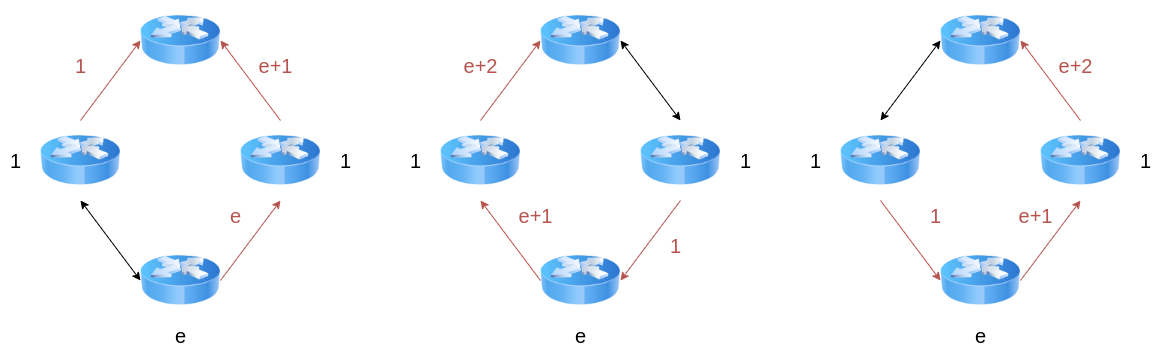
\includegraphics[width=330px]{images/5.1_Protocolli_di_routing/link_state_oscillation.png}
\end{figure}
questo comportamento si ha perché una volta creata una soluzione tutti i nodi iniziano ad applicarla, questo fa mutare enormemente i livelli di congestione, quindi si ha un ricalcolo delle routes.

\subsection{Distance Vector}
Si basano sul paradigma della programmazione dinamica.

\subsubsection{Bellman-Ford}
Supponiamo che $d_x(y)$ sia il costo minore possibile per andare da $x$ ad $y$, il nodo $x$ può trovare questo valore tramite:
$$ d_x(y) = min_v\{c(x,v) + d_v(y)\} $$
con:
\begin{itemize}
    \item $c(x,v)$: costo di andare da $x$ al suo vicino $v$
    \item $d_v(y)$: costo di andare dal vicino $v$ ad $y$
\end{itemize}
sostanzialmente noto l' elenco dei propri vicini, i costi per andare sui miei vicini e noti i costi che si hanno per andare dai miei vicini ad $y$ trovo il costo minimo per andare da me ad $y$.

Il nodo che mi minimizza questa distanza è quindi elevato a \emph{next-hop} ed utilizzato per instradare verso $y$:
$$ n* = arg min_v\{c(x,v) + d_v(y)\}$$

\subsubsection{Coordinazione e propagazione delle informazioni}
Questi tipi di algoritmi devono propagare le informazioni locali affinché ogni nodo possa computare le proprie route, eseguiamo quindi delle stime in successione:
chiamiamo $D_x(y)$ la stima del costo minimo per andare da $x$ ad $y$, il nodo $x$ mantiene in memoria il distance vector $D_x = [D_x(y):y \in N]$ cioè la stima dei costi minimi per andare da $x$ a tutti gli altri nodi della rete.

Ogni nodo $x$ conosce il costo preciso per andare su ogni suo vicino $v$: $c(x,v)$ e per ogni vicino mantiene il distance vector $D_v = [D_v(y): y \in N]$.

L' idea è quindi che ogni tanto ogni nodo spedisce ai propri vicini il proprio distance vector stimato.
Potrebbe avvenire periodicamente oppure su particolari eventi come forti mutazioni della congestione.
Ogni volta che ricevo un aggiornamento dei distance vector dei vicini lo uso assieme all' equazione di Bellman-Ford per aggiornare la mia distance vector:
$$ D_x(y) = min_v\{c(x,v) + D_v(y)\}, \forall y \in N $$

Sotto determinate condizioni la stima di $D_x(y)$ converge al reale costo minore $d_x(y)$.

\subsubsection{Algoritmo generico}
Il generico algoritmo di distance vector è iterativo, asincrono e distribuito.
Ogni nodo esegue:
\begin{enumerate}
    \item attesa di un cambiamento nei costi dei link con i vicini o di un messaggio dai vicini
    \item ricalcolo delle stime
    \item se la stima verso un vicino è cambiata glielo notifico
    \item ritornare ad 1
\end{enumerate}

\subsubsection{Problemi di Bellman-Ford}
Supponiamo che il costo su un arco diminuisca in questa maniera:
\begin{figure}[H]
    \centering
    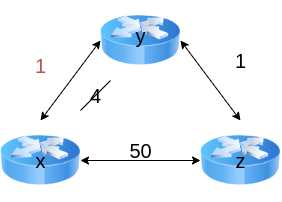
\includegraphics[width=150px]{images/5.1_Protocolli_di_routing/bellman_ford_change.png}
\end{figure}
in questo caso abbiamo che:
\begin{itemize}
    \item $y$ si accorge del cambiamento, aggiorna il suo distance vector ed informa i suoi vicini
    \item $Z$ riceve l' aggiornamento, aggiorna il suo distance vector per andare su $x$ e lo invia ai vicni
    \item $x$ riceve il nuovo distance vector da $z$, il suo distance vector non cambia quindi non propaga più
\end{itemize}
Supponiamo ora invece che il peso peggiori:
\begin{figure}[H]
    \centering
    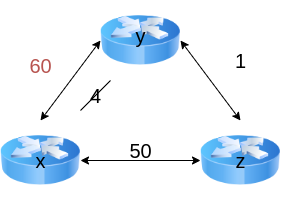
\includegraphics[width=150px]{images/5.1_Protocolli_di_routing/bellman_ford_problem_bad.png}
\end{figure}
in questo caso servono 44 iterazioni prima che l' algoritmo si stabilizzi, questo problema si chiama \emph{count to infinity}.

Es: $y$ conosce:
\begin{itemize}
    \item $D_y(x) = 4$
    \item $D_y(z) = 1$
    \item $D_z(y) = 1$
    \item $D_z(x) = 5$
    \item $c(y,x) = 4$
    \item $c(y,z) = 1$
\end{itemize}
quindi quando si accorge che ora $c(y,x)=60$, esegue i suoi calcoli con l' equazione di Bellman Ford e raggiunge la conclusione che:
$$D_y(x) = min\{(c(y,x)+D_x(x), c(y,z)+D_z(x)\} = min\{60+0, 1+5\} = 6$$
questa è una stima sbagliata ottenuta perché $y$ non ha la completa conoscenza della rete.
L' errore viene chiaramente tramandato perché ad ogni iterazione qualche distance vector cambia, in particolare ad ogni iterazione il costo viene incrementato di 1 finché il costo falso non supera quello vero ed allora la route cambia definitivamente e l' algoritmo si stabilizza.

Una soluzione (parziale) a questo problema è quello della \emph{poisoned reverse}: se il router $z$ instrada tramite $y$ per arrivare ad $x$ allora quando invierà il nuovo distance vector ad $y$ gli dirà che $D_z(x) = + \inf$, quindi $y$ non instraderà verso $z$ per andare su $x$.
Si noti che un problema di questo approccio è che $z$ non può sapere se $y$ proverà ad instradare verso $z$ stesso, questo problema causa il count to infinity.
Inoltre questo meccanismo di aggiornamento con questo problema causa un enorme traffico nella rete dovuto a tutti i pacchetti necessari per scambiarsi le informazioni.

\subsection{Comparazione tra LS e DV}
\subsubsection{Complessità del messaggio}
\begin{itemize}
    \item LS: dati $n$ nodi ed $E$ links abbiamo $O(nE)$ messaggi inviati
    \item DV: scambio di messaggi solo tra i vicini ma il tempo di convergenza varia
\end{itemize}

\subsubsection{Velocità di convergenza}
\begin{itemize}
    \item LS: $O(n^2)$ dell' algoritmo e richiede $O(nE)$ messaggi ma c'è la possibilità che si finisca in loop
    
    \item DV: il tempo di convergenza potrebbe variare, si potrebbero avere dei loop nel routing ed anche count-to-infinity
\end{itemize}

\subsubsection{Robustezza}
Cosa succede se un router ha un malfunzionamento:
\begin{itemize}
    \item LS: i nodi possono inviare costi dei link scorretti, inoltre ogni nodo si calcola la tabella solo per se quindi servono metodi per avvisare gli altri che la rete è cambiata
    
    \item DV: tramite la pubblicizzazione dei costi potrei avvisare i router con informazioni sbagliate, quindi gli errori si propagano attraverso la rete
\end{itemize}

\subsection{Routing gerarchico}
I router non sono identici e la rete non è piatta, singoli provider possono applicare delle politiche interne alla loro sottorete e non tutti i router devono conoscere/inviare proprie informazioni a tutti gli altri router della rete, sarebbe troppo traffico inutile.
Quello che si fa è quindi raggruppare assieme un tot di router costituendo un \emph{insieme autonomo} (autonomous system).

All' interno di questi sistemi si fa quel che si vuole, si usano gli algoritmi che si vuole, insomma una autonomia amministrativa.
Internamente al sistema ovviamente si usa lo stesso protocollo di routing, si parla di \emph{intra-AS routing}.
All' interno di questi sitemi si inseriscono poi dei \emph{gateway router} che permettono di comunicare con altri autonomous system.

Le tabelle di routing quindi sono riempite sia dagli algoritmi di Intra-AS routing che dagli algoritmi di Inter-AS routing.
In particolare le entry della tabella gestite dall' Intra-AS routing contengono il next-hop nel caso in cui si debba fare forwarding di pachetti nella stessa AS, mentre le etry dell' Inter-AS routing contengono il next-hop per l' uscita dall' AS con minor costo.

I router gateway di un AS devono scoprire quali destinazioni sono raggiungibili tramite gli altri AS ai quali sono connessi, una volta fatto ciò devono metterne al corrente tutti i router dell' AS.

\subsection{Intra-AS routing}
Detto anche Interior Gateway Protocols (IGP) si basa su 2 protocolli principali:
\begin{itemize}
    \item RIP: Routing Information Protocol
    \item OSPF: Open Shortest Path First
\end{itemize}

\subsubsection{RIP}
E' incluso in BSD-UNIX dal 1982, utilizza un algoritmo di distance vector.
Come metrica usa il numero di hop quindi ogni link ha costo unitario, così facendo non abbiamo il problema del count-to-infinity.

L' advertising del DV è eseguito ogni 30s ed ogni messaggio di advertising è una lista contenente fino a 25 sottoretti di destinazione.

\subsubsection{OSPF}
E' un protocollo di tipo link state, open nel senso che è pubblicamente disponibile.
La computazione dello shortest path è generata attraverso l' algoritmo di Dijkstra.
L' advertisement di OSPF contiene una entry per ogni vicino e l' advertisement è floodato all' intera AS direttamente attraverso IP.

Anche OSPF è gerarchico, in particolare suddividiamo un AS in varie aree ed ogni area ha le sue iterazioni di OSPF.
Così facendo il flooding comporta meno traffico nella rete in quanto ci sono meno router.
Quando si vuole andare all' esterno si contattano i router di boundary.
L' area intermedia tra le singole aree OSPF ed il router di gateway (o boundary) è detta \emph{backbone} (dorsale):
\begin{figure}[H]
    \centering
    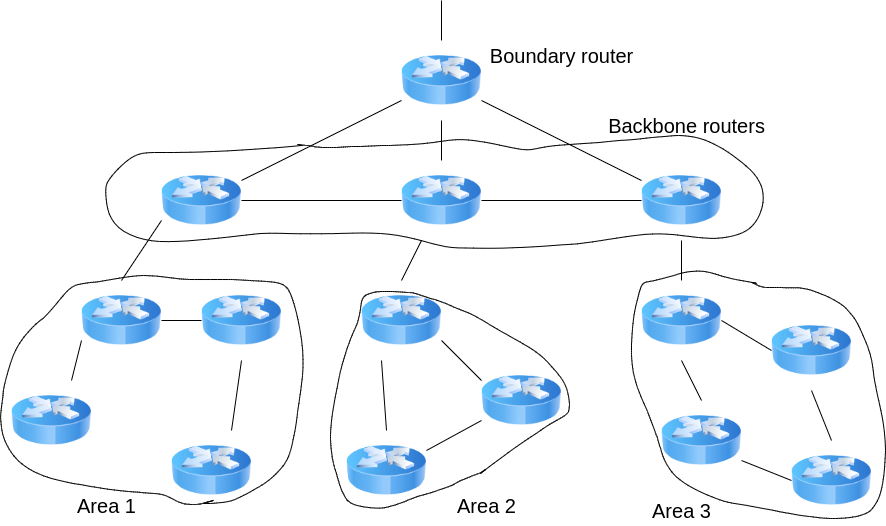
\includegraphics[width=300px]{images/5.1_Protocolli_di_routing/hierarchical_ospf.png}
\end{figure}
Si costruisce una gerarchia a due livelli: local area e backbone.
L' advertisement del link state è eseguito solo nell' area ed ogni nodo ha i dettagli della topologia dell' area, cioè conosce i percorsi brevi verso le reti nelle altre aree. 
I router nella backbone invece eseguono OSPF limitato alla backbone mentre i boundary routers connettono ad altre AS.

In definitiva: se si deve instradare qualche pacchetto in una rete interna alla AS si usano le route inserite da OSPF, se si deve instradare traffico verso reti esterne alla AS si invia il traffico direttamente al boundary router.

\subsection{Inter-AS routing}
Ci permette di creare le tabelle di routing tra le diverse AS, i protocolli di questa famiglia sono eseguiti solamente sui router di frontiera delle AS.

\subsubsection{BGP}
Il BGP - Border Gateway Protocol è lo standard de-facto per il router inter-domain: \emph{è la colla che tiene Internet insieme}.
BGP ci permette di:
\begin{itemize}
    \item eBGP (external BGP): ottenere le subnet raggiungibili attraverso le AS vicine
    \item iBGP (internal BGP): propagare le informazioni sulle subnet raggiungibili a tutti i router interni della AS
    \item determinare router buone verso altre reti in base alle informazioni di reachability e varie policy specifiche
\end{itemize}
Possiamo quindi istruire le subnet a fare advertisement in modo che possano dichiarare la loro posizione attraverso Internet.

Alcuni esempi di policy che possono essere portate avanti da BGP sono: una AS aziendale potrebbe non essere disposta a trasportare pacchetti generati da un AS estraneo e diretti ad un altro AS estraneo anche se si trova sullo shortest path, oppure trasmetterli se e solo se hanno pagato il servizio (servizio di transito), ecc ecc.

Queste politche di routing possono essere proprietarie ed individuali (quindi decise dal gestore della AS) e permettono di decidere quale traffico può fluire su quali linee fra le varie AS.

Il protocollo si serve delle cosidette BGP session: due router BGP si scambiano messaggi BGP per fare advertising dei percorsi verso diverse reti di destinazione, si parla di protocollo \emph{path vector} proprio perché si parla di percorso e non di distanza.
Quando un AS fa l' advertising  di un prefisso ad un' altra AS \emph{promette} di instradare il traffico verso quel prefisso se dovesse arrivargli.

Per rendere più efficiente l' advertising ogni AS può aggregare diversi prefissi per crearne di più grandi se ne ha la possibilità.

Una volta che eBGP fa l' advertising sugli altri gateway router il gateway esegue l' advertising all' interno della AS usando iBGP, in questo modo i router interni nell' AS sono messi a conoscenza dei percorsi per raggiungere le nuove reti.
Tramite iBGP inoltre i router di boundary della stessa AS comunicano tra di loro e quindi propagano l' advertisement ad alte AS.

Nell' advertisement oltre al prefix della rete raggiungibile si aggiungono \emph{attributi}:
\begin{itemize}
    \item AS-PATH: contiene l' elenco delle AS attraversate dall' advertisement
    \item NEXT-HOP: indica il router interno all' AS al quale inoltrare per uscire e seguire il path indicato da AS-PATH (contiene l' indirizzo IP del router di boundary dal quale è entrato l' advertisement)
\end{itemize}
inoltre applicano le policy di cui abbiamo discusso in precedenza per non propagare eventuali advertisement.

Se il router riceve diversi advertisement per la stessa destinazione si possono scegliere le route sulla base di:
\begin{itemize}
    \item preferenze locali in base alle policy impostate
    \item il più vicino AS-PATH
    \item il router NEXT-HOP più vicino (hot potato routing)
    \item eventuali altri criteri
\end{itemize}

\subsection{Come si riempie la tabella di routing?}
\begin{enumerate}
    \item il router viene a conoscenza dei prefissi raggiungibili attraverso l'advertisement dei prefissi via BGP
    \item il router determina la porta sulla quale instradare per raggiungere il prefisso: si usa la selezione delle route BGP per trovare la migliore route inter-AS.
    Successivamente si usano protocolli di intra-AS per trovare i percorsi migliori all' interno della stessa AS, quindi si ottiene la porta del router che da su questa route.
    \item si aggiunge la coppia $<$prefisso,porta$>$ alla tabella di routing
\end{enumerate}

\subsection{Perché distinguere tra Intra-AS ed Inter-AS?}
Per avere una migliore granularità nell applicazione delle policy.
Il gestore della AS può voler poter usare delle diverse politiche rispetto ai gestori delle altre AS.
Conviene da un punto di vista tecnico per creare delle gerarchie, diminuire le dimensioni delle tabelle di routing del singolo router, diminuire il tempo necessario per l' aggiornamento.

Inoltre gli algoritmi di Intra-AS possono concentrarsi sull' efficienza mentre quelli di Inter-AS possono soprassedere queste valutazioni per raggiungere lo scopo.
